%package list
\documentclass{article}
\usepackage[top=3cm, bottom=3cm, outer=3cm, inner=3cm]{geometry}
\usepackage{multicol}
\usepackage{graphicx}
\usepackage{url}
%\usepackage{cite}
\usepackage{hyperref}
\usepackage{array}
%\usepackage{multicol}
\newcolumntype{x}[1]{>{\centering\arraybackslash\hspace{0pt}}p{#1}}
\usepackage{natbib}
\usepackage{pdfpages}
\usepackage{multirow}
\usepackage[normalem]{ulem}
\useunder{\uline}{\ul}{}
\usepackage{svg}
\usepackage{xcolor}
\usepackage{listings}
\lstdefinestyle{ascii-tree}{
    literate={├}{|}1 {─}{--}1 {└}{+}1 
  }
\lstset{basicstyle=\ttfamily,
  showstringspaces=false,
  commentstyle=\color{red},
  keywordstyle=\color{blue}
}
%\usepackage{booktabs}
\usepackage{caption}
\usepackage{subcaption}
\usepackage{float}
\usepackage{array}

\newcolumntype{M}[1]{>{\centering\arraybackslash}m{#1}}
\newcolumntype{N}{@{}m{0pt}@{}}


%%%%%%%%%%%%%%%%%%%%%%%%%%%%%%%%%%%%%%%%%%%%%%%%%%%%%%%%%%%%%%%%%%%%%%%%%%%%
%%%%%%%%%%%%%%%%%%%%%%%%%%%%%%%%%%%%%%%%%%%%%%%%%%%%%%%%%%%%%%%%%%%%%%%%%%%%
\newcommand{\itemEmail}{fgarambel@unsa.edu.pe}
\newcommand{\itemStudent}{Fernando Miguel Garambel Marín}
\newcommand{\itemCourse}{Laboratorio de Programación Web 2}
\newcommand{\itemCourseCode}{1701212}
\newcommand{\itemSemester}{III}
\newcommand{\itemUniversity}{Universidad Nacional de San Agustín de Arequipa}
\newcommand{\itemFaculty}{Facultad de Ingeniería de Producción y Servicios}
\newcommand{\itemDepartment}{Departamento Académico de Ingeniería de Sistemas e Informática}
\newcommand{\itemSchool}{Escuela Profesional de Ingeniería de Sistemas}
\newcommand{\itemAcademic}{2024 - A}
\newcommand{\itemInput}{Del 24 de mayo 2024}
\newcommand{\itemOutput}{Al 14 de junio 2024}
\newcommand{\itemPracticeNumber}{08}
\newcommand{\itemTheme}{Django: Relaciones de uno a muchos, muchos a muchos y impresión de pdf y emails}
%%%%%%%%%%%%%%%%%%%%%%%%%%%%%%%%%%%%%%%%%%%%%%%%%%%%%%%%%%%%%%%%%%%%%%%%%%%%
%%%%%%%%%%%%%%%%%%%%%%%%%%%%%%%%%%%%%%%%%%%%%%%%%%%%%%%%%%%%%%%%%%%%%%%%%%%%

\usepackage[english,spanish]{babel}
\usepackage[utf8]{inputenc}
\AtBeginDocument{\selectlanguage{spanish}}
\renewcommand{\figurename}{Figura}
\renewcommand{\refname}{Referencias}
\renewcommand{\tablename}{Tabla} %esto no funciona cuando se usa babel
\AtBeginDocument{%
	\renewcommand\tablename{Tabla}
}

\usepackage{fancyhdr}
\pagestyle{fancy}
\fancyhf{}
\setlength{\headheight}{30pt}
\renewcommand{\headrulewidth}{1pt}
\renewcommand{\footrulewidth}{1pt}
\fancyhead[L]{\raisebox{-0.2\height}{
\includegraphics[width=3cm]{img/logo_episunsa.png}}}
\fancyhead[C]{\fontsize{7}{7}\selectfont	\itemUniversity \\ \itemFaculty \\ \itemDepartment \\ \itemSchool \\ \textbf{\itemCourse}}
\fancyhead[R]{\raisebox{-0.2\height}{
\includegraphics[width=1.2cm]{img/logo_abet}}}
\fancyfoot[L]{Fernando Garambel}
\fancyfoot[C]{\itemCourse}
\fancyfoot[R]{Página \thepage}

% para el codigo fuente
\usepackage{listings}
\usepackage{color, colortbl}
\definecolor{dkgreen}{rgb}{0,0.6,0}
\definecolor{gray}{rgb}{0.5,0.5,0.5}
\definecolor{mauve}{rgb}{0.58,0,0.82}
\definecolor{codebackground}{rgb}{0.95, 0.95, 0.92}
\definecolor{tablebackground}{rgb}{0.8, 0, 0}

\lstset{frame=tb,
	language=bash,
	aboveskip=3mm,
	belowskip=3mm,
	showstringspaces=false,
	columns=flexible,
	basicstyle={\small\ttfamily},
	numbers=none,
	numberstyle=\tiny\color{gray},
	keywordstyle=\color{blue},
	commentstyle=\color{dkgreen},
	stringstyle=\color{mauve},
	breaklines=true,
	breakatwhitespace=true,
	tabsize=3,
	backgroundcolor= \color{codebackground},
}

\begin{document}
	
	\vspace*{10px}
	
	\begin{center}	
		\fontsize{17}{17} \textbf{ Informe de Laboratorio \itemPracticeNumber}
	\end{center}
	\centerline{\textbf{\Large Tema: \itemTheme}}
	%\vspace*{0.5cm}	

	\begin{flushright}
		\begin{tabular}{|M{2.5cm}|N|}
			\hline 
			\rowcolor{tablebackground}
			\color{white} \textbf{Nota}  \\
			\hline 
			     \\[30pt]
			\hline 			
		\end{tabular}
	\end{flushright}	

	\begin{table}[H]
		\begin{tabular}{|x{4.7cm}|x{4.8cm}|x{4.8cm}|}
			\hline 
			\rowcolor{tablebackground}
			\color{white} \textbf{Estudiante} & \color{white}\textbf{Escuela}  & \color{white}\textbf{Asignatura}   \\
			\hline 
			{\itemStudent \par \itemEmail} & \itemSchool & {\itemCourse \par Semestre: \itemSemester \par Código: \itemCourseCode}     \\
			\hline 			
		\end{tabular}
	\end{table}		
	
	\begin{table}[H]
		\begin{tabular}{|x{4.7cm}|x{4.8cm}|x{4.8cm}|}
			\hline 
			\rowcolor{tablebackground}
			\color{white}\textbf{Laboratorio} & \color{white}\textbf{Tema}  & \color{white}\textbf{Duración}   \\
			\hline 
			\itemPracticeNumber & \itemTheme & 04 horas   \\
			\hline 
		\end{tabular}
	\end{table}
	
	\begin{table}[H]
		\begin{tabular}{|x{4.7cm}|x{4.8cm}|x{4.8cm}|}
			\hline 
			\rowcolor{tablebackground}
			\color{white}\textbf{Semestre académico} & \color{white}\textbf{Fecha de inicio}  & \color{white}\textbf{Fecha de entrega}   \\
			\hline 
			\itemAcademic & \itemInput &  \itemOutput  \\
			\hline 
		\end{tabular}
	\end{table}

\section{Objetivos}
	\begin{itemize}		
		\item Implementar en una aplicación en Django el manejo de Bases de datos.
		\item	Utilizar una tabla y relacionarla con muchas tablas.
		\item Utilizar muchas tablas y relacionarlas con muchas tablas.
		\item Implementar el envío de emails y la impresión de pdfs desde una aplicación Django
	\end{itemize}
\section{Actividades}
	\begin{itemize}		
		\item Crear un proyecto en Django
		\item Siga los pasos de los videos para poder implementar la aplicación de Relación de Uno a muchos en una Base de Datos, muchos a muchos, impresión de pdfs y envío de emails.
		\item Use git y haga los commits necesarios para manejar correctamente la aplicación.
	\end{itemize}
\section{Ejercicio Propuestos}
	\begin{itemize}		
		\item Deberán replicar la actividad de los videos donde se trabaja con Relacion de uno a muchos, de muchos a muchos, impresión de pdfs y envío de emails;  adecuándolo desde un proyecto en blanco Django.
		\item Para ello crear una carpeta dentro del proyecto github colaborativo con el docente, e informar el link donde se encuentra.
		\item	Eres libre de agregar CSS para decorar tu trabajo.
		\item Ya sabes que el trabajo con Git es obligatorio.  Revisa los videos entregados.
	\end{itemize}
\section{Equipos, materiales y temas utilizados}
	\begin{itemize}
		\item Sistema operativo de 64 bits, procesador basado en x64.
		\item Latex. 
		\item git version 2.41.0.windows.1
		\item Cuenta en GitHub con el correo institucional.
	\end{itemize}
\section{URL Github, Video}
	\begin{itemize}
		\item URL del Repositorio GitHub para clonar o recuperar.
		\item \url{https://github.com/FernandoGarambelM/Lab08_Django_relaciones.git}
		\item URL para el video flipgrid
		\item \url{https://flip.com/s/pvZBG1NhvCRn}	
	\end{itemize}
	\clearpage
\section{Replicando la actividad del video}
	\begin{itemize}
		\item Primero ingresamos al entorno virtual
	\end{itemize}
	\begin{lstlisting}[language=bash,caption={Activar el ambiente virtual}][H]
		env\Scripts\activate
	\end{lstlisting}
	\begin{lstlisting}[language=bash,caption={Clonar el repositorio}][H]
		git clone https://github.com/navinreddy20/django-telusko-codes
	\end{lstlisting}
	\begin{itemize}
		\item Luego instalamos postgresql y pgadmin 
		\item Luego instalamos al entorno virtual psycopg2-binary y Pillow
	\end{itemize}
	\begin{lstlisting}[language=bash,caption={Instalando psycopg2-binary y Pillow}][H]
		pip install psycopg2-binary
		pip install Pillow
	\end{lstlisting}
	\begin{itemize}
		\item  Despues de instalar, creamos un superusuario con el siguiente script
	\end{itemize}
\begin{lstlisting}[language=bash,caption={Script para crear un superusuario}][H]

#!/bin/sh

# Variables de entorno para el superusuario
DJANGO_SUPERUSER_USERNAME=admin
DJANGO_SUPERUSER_EMAIL=admin@example.com
DJANGO_SUPERUSER_PASSWORD=123456

# Ejecutar el comando createsuperuser sin interaccion
python manage.py shell -c "from django.contrib.auth import get_user_model; User = get_user_model(); User.objects.create_superuser('$DJANGO_SUPERUSER_USERNAME', '$DJANGO_SUPERUSER_EMAIL', '$DJANGO_SUPERUSER_PASSWORD') if not User.objects.filter(username='$DJANGO_SUPERUSER_USERNAME').exists() else print('Superusuario ya existe.')"
	\end{lstlisting}
	\begin{itemize}
		\item Realizamos migraciones para enlazar la base de datos
	\end{itemize}
	\begin{lstlisting}[language=bash,caption={Codigo para realizar migraciones}][H]
		python manage.py makemigrations
		python manage.py migrations
	\end{lstlisting}
	\begin{itemize}
		\item Despues de seguir estos pasos la plantilla ya funciona por completo
	\end{itemize}
\section{Adecuar la plantilla a un proyecto en blanco de Django}
	\begin{itemize}
		\item Creamos el modelo destination con los datos requeridos
	\end{itemize}
\lstinputlisting[language=Python, caption={Código de models.py},numbers=left,]{src/models1.py}
	\begin{itemize}
\section{Crear formularios de Añadir Destinos Turísticos, Modificar, Listar y Eliminar Destinos. }
		\item Luego creamos los forms 
	\end{itemize}
\lstinputlisting[language=Python, caption={Código de forms.py},numbers=left,]{src/forms.py}
	\begin{itemize}
		\item Luego creamos views.py
	\end{itemize}	
\lstinputlisting[language=Python, caption={Código de views.py},numbers=left,]{src/views.py}
	\begin{itemize}
		\item Luego agregamos urls.py para que Django pueda leerlos
	\end{itemize}	
\lstinputlisting[language=Python, caption={Código de urls.py},numbers=left,]{src/urls.py}	
	\begin{itemize}
		\item Usamos la  plantilla de travello, especificamente la siguiente parte para listar los destinos turisticos con if y for
	\end{itemize}	
	\begin{lstlisting}[language=bash,caption={Pedazo de html donde se usa  for e if}][H]
						
							<!-- Destination -->
							<div class="destination item">
								<div class="destination_image">
									<img src="{{dest.img.url}}" alt="">

									
									<div class="spec_offer text-center"><a href="#">Special Offer</a></div>
									
								</div>
								<div class="destination_content">
									<div class="destination_title"><a href="destinations.html">{{dest.name}}</a>
									</div>
									<div class="destination_subtitle">
										<p>{{dest.desc}}</p>
									</div>
									<div class="destination_price">From ${{dest.price}}</div>
								</div>
							</div>

							

	\end{lstlisting}
	\begin{itemize}
		\item Se crea en templates gestionar destinos.html
	\end{itemize}	
	\begin{lstlisting}[language=bash,caption={Html de gestionar destinos.html}][H]

<!DOCTYPE html>
<html>
<head>
    <title>Gestionar Destinos</title>
    <link rel="stylesheet" type="text/css" href="">
</head>
<body>
    <h1>Gestionar Destinos Turisticos</h1>
    
    <!-- Formulario de Aniadir/Modificar -->
    <form method="post" enctype="multipart/form-data">
        
        {{ form.as_p }}
        <button type="submit" name="modificar" disabled>Modificar</button>
        <button type="submit" name="eliminar" disabled>Eliminar</button>
        <button type="submit" name="aniadir" disabled>Anadir</button>
    </form>
    
    <h2>Lista de Destinos</h2>
    <ul>
        
            <li>
                <h2>{{ destino.name }}</h2>
                <p>{{ destino.desc}}</p>
                <p>Precio: {{ destino.price}}</p>
                <p>En oferta</p>
                <a href="">Seleccionar</a>
            </li>
        
    </ul>
    
</body>
</html>
	\end{lstlisting}
	\begin{itemize}
		\item Para el registro y login de usuarios hacemos los mismo pasos para crear la app y ahora mostramos solo views por que es lo mas importante
	\end{itemize}	
	\begin{lstlisting}[language=Python,caption={Codigo de views.py de accounts}][H]
from django.shortcuts import render, redirect
from django.contrib import messages
from django.contrib.auth.models import User, auth

# Create your views here.
def login(request):
    if request.method== 'POST':
        username = request.POST['username']
        password = request.POST['password']

        user = auth.authenticate(username=username,password=password)

        if user is not None:
            if user.is_superuser:
                auth.login(request, user)
                return redirect("/gestionar")   
            else:
                auth.login(request, user)
                return redirect("/")
        else:
            messages.info(request,'invalid credentials')
            return redirect('login')

    else:
        return render(request,'login.html')    

def register(request):

    if request.method == 'POST':
        first_name = request.POST['first_name']
        last_name = request.POST['last_name']
        username = request.POST['username']
        password1 = request.POST['password1']
        password2 = request.POST['password2']
        email = request.POST['email']

        if password1==password2:
            if User.objects.filter(username=username).exists():
                messages.info(request,'Username Taken')
                return redirect('register')
            elif User.objects.filter(email=email).exists():
                messages.info(request,'Email Taken')
                return redirect('register')
            else:   
                user = User.objects.create_user(username=username, password=password1, email=email,first_name=first_name,last_name=last_name)
                user.save();
                print('user created')
                return redirect('login')

        else:
            messages.info(request,'password not matching..')    
            return redirect('register')
        return redirect('/')
        
    else:
        return render(request,'register.html')


def logout(request):
    auth.logout(request)
    return redirect('/')       
	\end{lstlisting}
	\begin{itemize}
		\item Aqui se procesan los datos obtenidos en login y register
	\end{itemize}	
\lstinputlisting[language=html, caption={Código de login.html},numbers=left,]{src/login.html}	
\lstinputlisting[language=html, caption={Código de register.html},numbers=left,]{src/register.html}	
\section {Resultado}
	\begin{itemize}
		\item Lista de los destinos turisticos
	\end{itemize}	
	\begin{figure}[H]
		\centering
		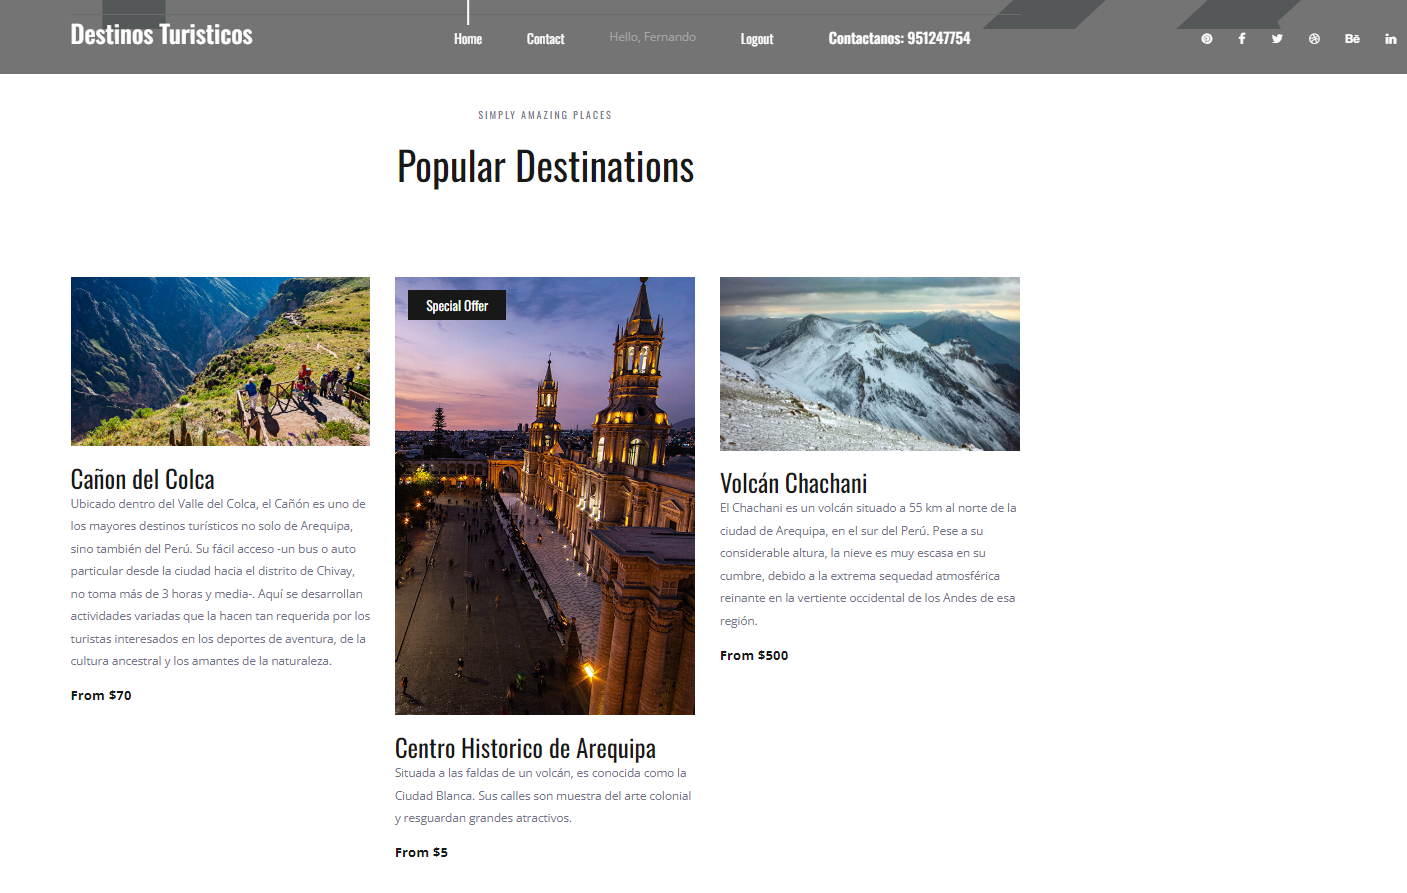
\includegraphics[width=1.0\textwidth,keepaspectratio]{img/Vista1.png}
		%\includesvg{img/automata.svg}
		%\label{img:mot2}
		%\caption{Product backlog.}
	\end{figure}
	\begin{itemize}
		\item Vista de los forms para gestionar los diferentes destinos turisticos
	\end{itemize}	
	\begin{figure}[H]
		\centering
		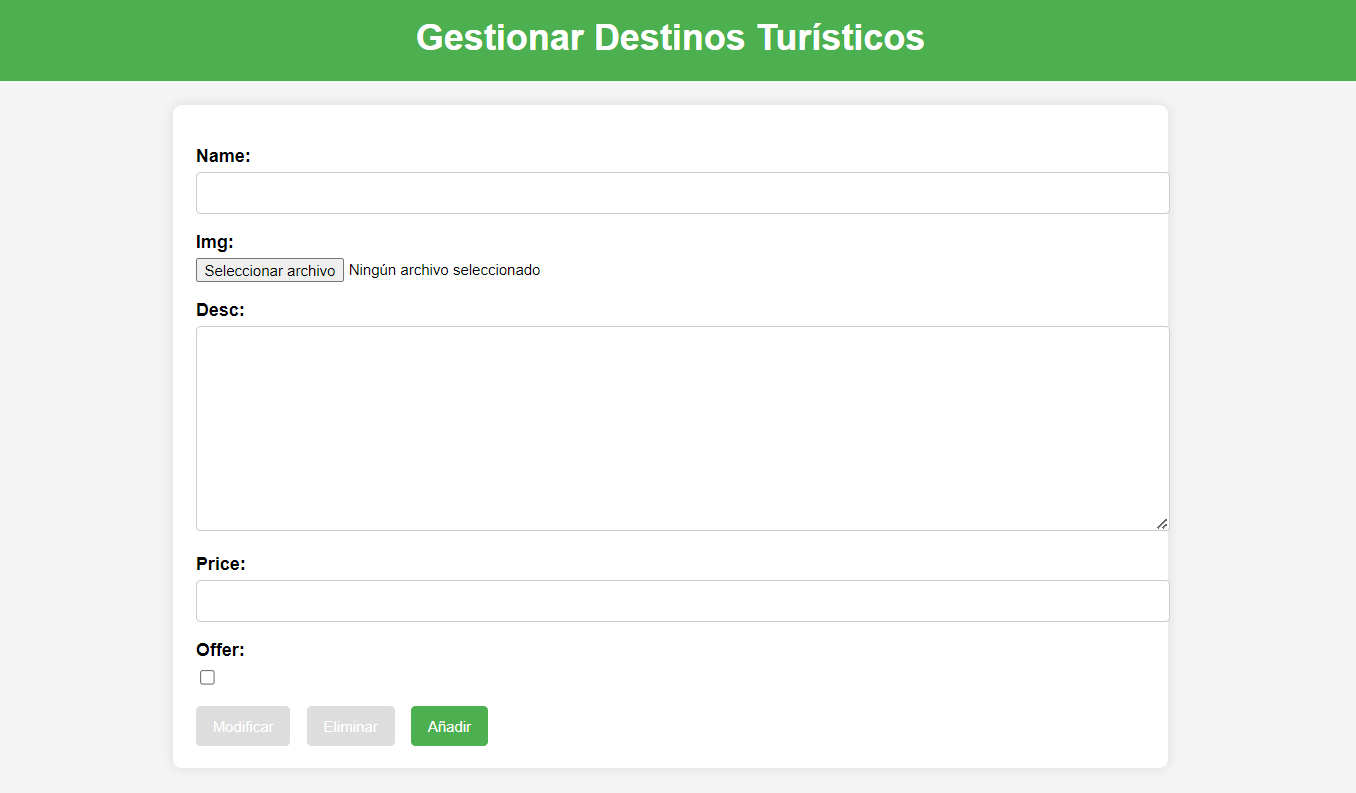
\includegraphics[width=1.0\textwidth,keepaspectratio]{img/Vista3.png}
		%\includesvg{img/automata.svg}
		%\label{img:mot2}
		%\caption{Product backlog.}
	\end{figure}
	\begin{figure}[H]
		\centering
		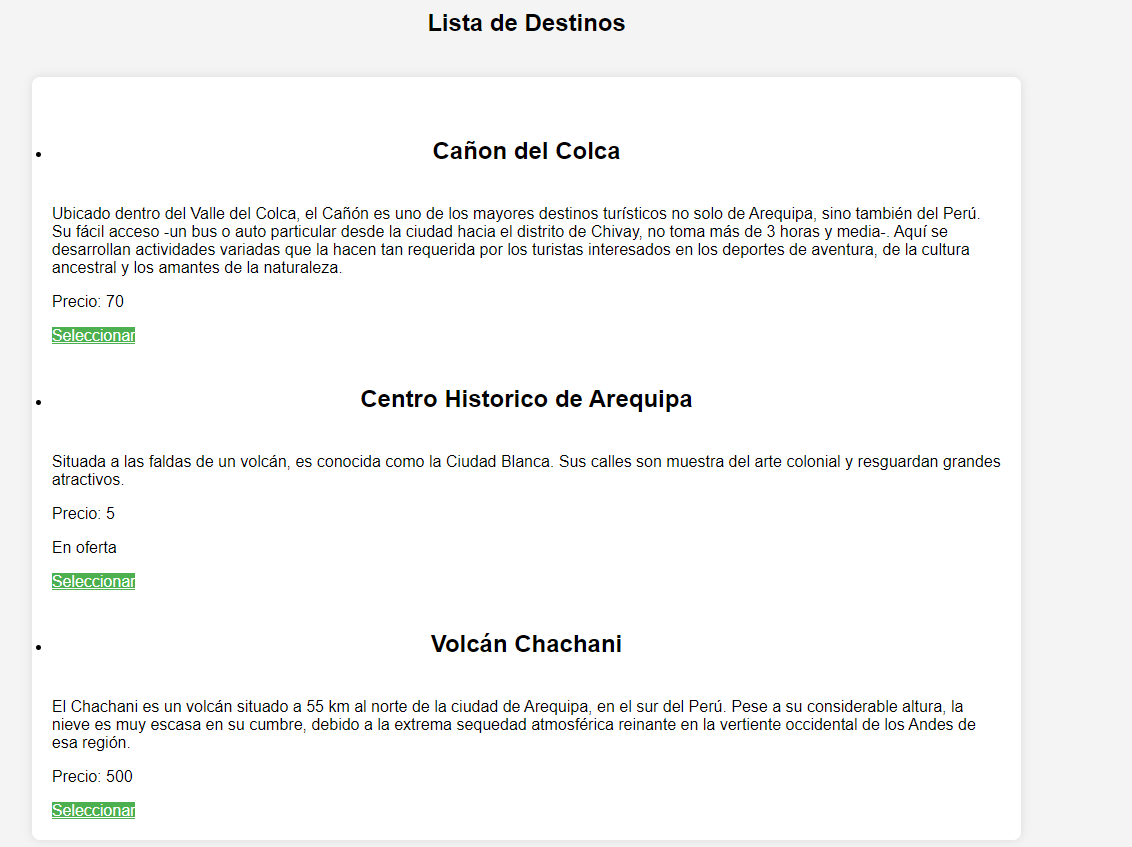
\includegraphics[width=1.0\textwidth,keepaspectratio]{img/Vista4.png}
		%\includesvg{img/automata.svg}
		%\label{img:mot2}
		%\caption{Product backlog.}
	\end{figure}
\section{Referencias}
\begin{itemize}			
	\item \url{https://docs.djangoproject.com/es/3.2/}
	\item\url{https://docs.djangoproject.com/es/3.2/ref/models/fields/#field-types}
\end{itemize}	
	
%\clearpage
%\bibliographystyle{apalike}
%\bibliographystyle{IEEEtranN}
%\bibliography{bibliography}
			
\end{document}